\subsubsection{Comando GET}
Nel messaggio di comando get, i primi 8 bit che specificano il comando sono 
seguiti dal nome del file che si vuole scaricare, questo campo è composto da un 
numero indefinito di byte, che il server lo interpreta come una stringa, 
pertanto legge carattere per carattere fintanto che non trova il terminatore.
%	+-------+-----------------------+
%	|  GET  |	   file_name     	|
%	+-------+-----------------------+
%  	  8 bit
\begin{figure}[!h]
	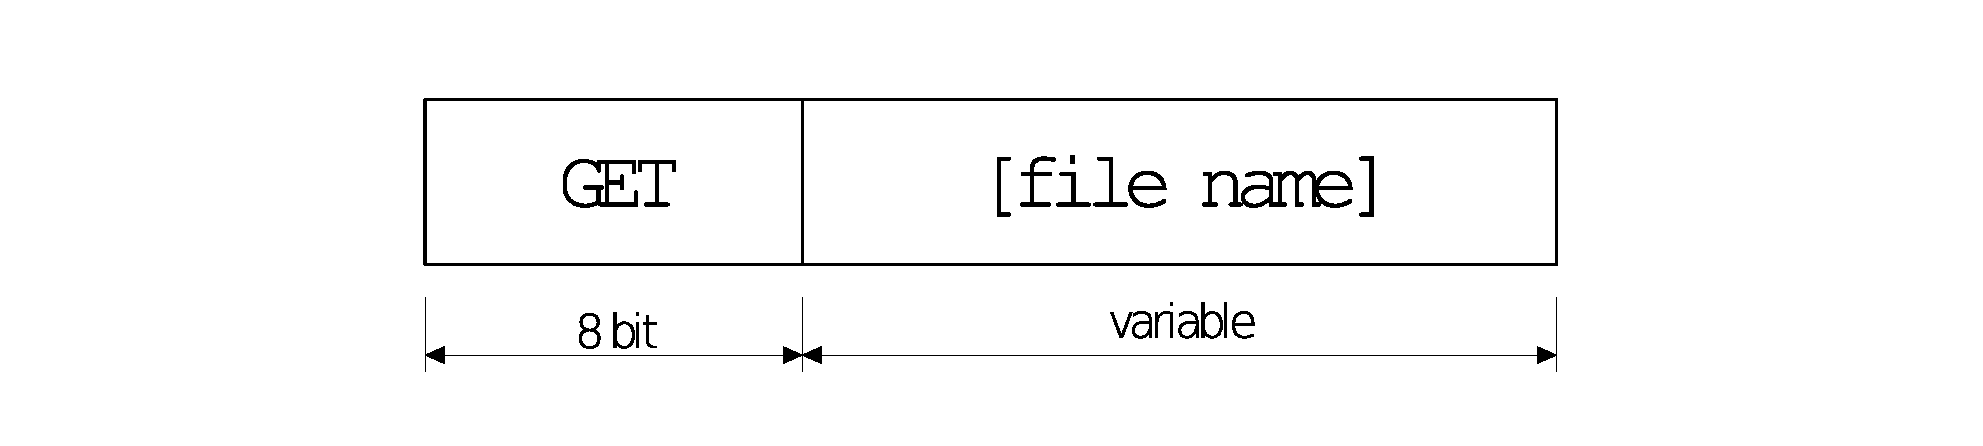
\includegraphics[scale=0.35]{images/get_client}
	\caption{Messaggio di comando GET}
\end{figure}
Il server una volta ottenuto il nome del file, controlla se è presente in memoria e, in caso affermativo, prepara il messaggio di risposta così strutturato:
i primi 8 bit contengono una costante che indica che il file esiste, i successivi 64 bit la dimensione del file, infine segue l'intero file.
%+---------+-------------------------+---------------------------+
%| GET_OK  |	       file_size        |	..		file		..	|
%+---------+-------------------------+---------------------------+
%  8 bit				64 bit
\begin{figure}[!h]
	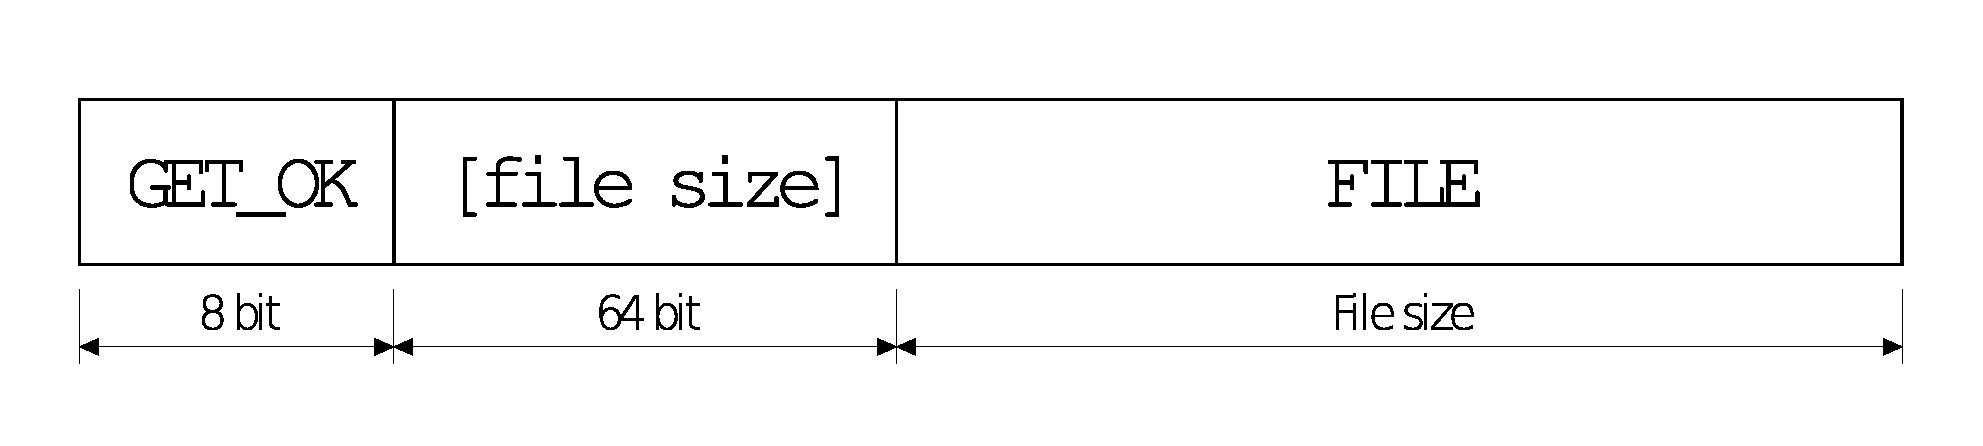
\includegraphics[scale=0.35]{images/get_server_ok}
	\caption{Messaggio di risposta GET}
\end{figure}
Se il file non esiste, viene inviato un messaggio di soli 8 bit contente la costante che ne indica l'assenza.
%+-----------+
%| GET_NOENT |
%+-----------+
%  	8 bit
\begin{figure}[!h]
	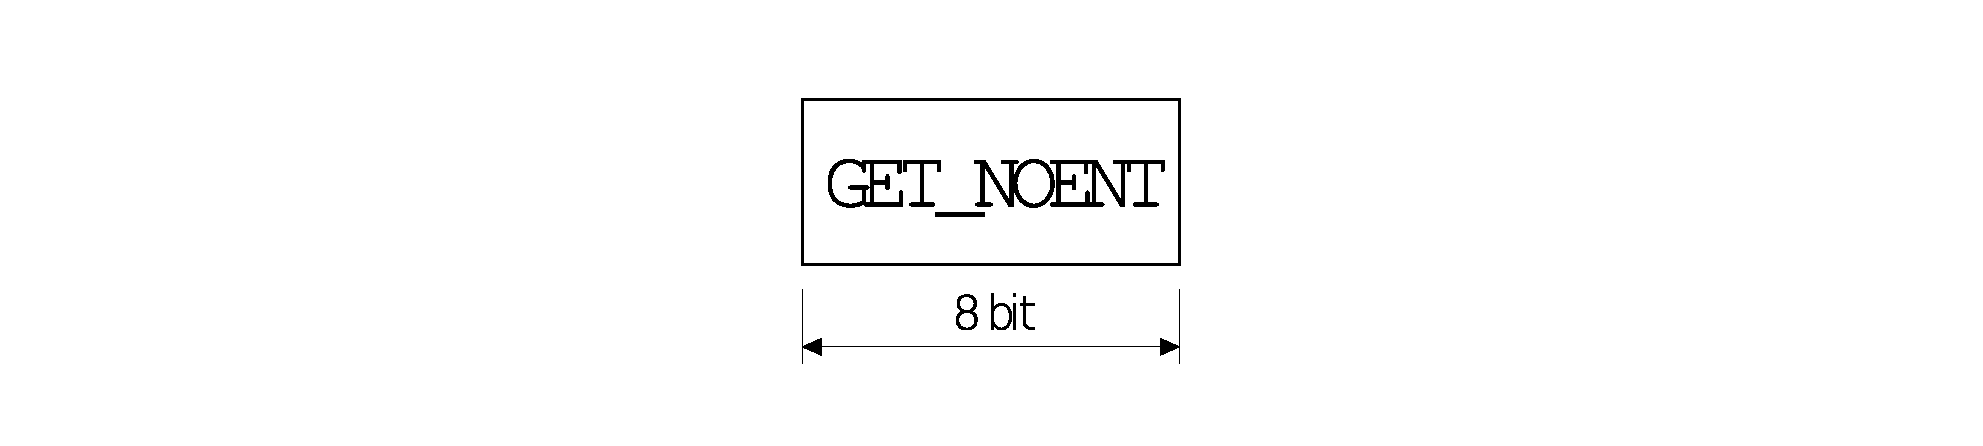
\includegraphics[scale=0.35]{images/get_server_noent}
	\caption{Messaggio di risposta GET}
\end{figure}
